\documentclass[11pt]{article}
\pdftrailerid{}
\usepackage[T1]{fontenc}
\usepackage{lmodern}
\usepackage[margin=1.05in]{geometry}
\usepackage{amsmath,amssymb,amsthm,mathtools,microtype}
\usepackage{enumitem,xcolor,tikz}
\usetikzlibrary{arrows.meta,calc,positioning,patterns}
\usepackage[colorlinks=true,linkcolor=blue!45!black,citecolor=blue!45!black,urlcolor=blue!45!black]{hyperref}
\setlength{\emergencystretch}{2em}
\setlist{itemsep=3pt,topsep=5pt}
\newcommand{\C}{\mathbb C}
\newcommand{\R}{\mathbb R}
\newcommand{\Z}{\mathbb Z}
\newcommand{\N}{\mathbb N}
\newcommand{\T}{(\C^\times)^2}
\newcommand{\PP}{\mathbb P}
\DeclareMathOperator{\conv}{conv}
\DeclareMathOperator{\ord}{ord}
\DeclareMathOperator{\mult}{mult}
\DeclareMathOperator{\Span}{span}
\DeclareMathOperator{\rk}{rank}
\DeclareMathOperator{\codim}{codim}
\DeclareMathOperator{\id}{id}
\newtheorem{theorem}{Theorem}[section]
\newtheorem{lemma}[theorem]{Lemma}
\newtheorem{proposition}[theorem]{Proposition}
\newtheorem{corollary}[theorem]{Corollary}
\theoremstyle{definition}
\newtheorem{definition}[theorem]{Definition}
\newtheorem{remark}[theorem]{Remark}
\numberwithin{equation}{section}
\hypersetup{pdftitle={Maximal Seshadri constants on arbitrary polarized surfaces},pdfauthor={OpenAI}}

\title{Maximal Seshadri constants on arbitrary polarized surfaces}
\author{OpenAI}
\date{September 23, 2026}
\begin{document}
\maketitle
\begin{abstract}
We prove that, for every smooth integral complex projective surface $S$
and every ample line bundle $L$, the multipoint Seshadri constant at $r$
very general points equals $\sqrt{L^2/r}$ for every sufficiently large
integer $r$. This resolves positively the qualitative Nagata--Biran
conjecture for surfaces. The proof combines finite jet interpolation near
a nodal curve with torus subgroups of prescribed order.
\end{abstract}
\tableofcontents
\section{Introduction}\label{sec:introduction}

Let $S$ be a smooth integral complex projective surface and $L$ an ample
line bundle. We use additive notation for tensor powers and put $H=L^2$.
For a tuple of distinct points $\mathbf p=(p_1,\ldots,p_r)$, the multipoint
Seshadri constant is
\[
 \varepsilon(S,L;\mathbf p)
 =\inf_C\frac{L\cdot C}{\sum_{i=1}^r\mult_{p_i}C},
\]
where $C$ ranges over integral curves meeting at least one of the points.
If $\pi:Y\to S$ is the blow-up of these points, with exceptional curves
$E_1,\ldots,E_r$, the same constant is the largest $\lambda\ge0$ for
which $\pi^*L-\lambda\sum_iE_i$ is nef. Here a real divisor class is
\emph{nef} if it has nonnegative intersection with every integral curve.
This constant measures how much of the positivity of $L$ remains after
subtracting equal exceptional weights at the chosen points. Its universal
bound is
\begin{equation}\label{eq:upper-bound}
 \varepsilon(S,L;\mathbf p)\le\sqrt{\frac Hr};
\end{equation}
an elementary jet-count proof appears in Lemma~\ref{lem:sesha-upper}.

Write
\[
 U_r=\{(p_1,\ldots,p_r)\in S^r:p_i\ne p_j\text{ for }i\ne j\}.
\]
A property holds at \emph{very general} tuples if its failures are contained
in a countable union of proper Zariski-closed subsets of $U_r$.

\begin{theorem}\label{thm:main}
For every smooth integral complex projective surface $S$ and every ample
line bundle $L$ on $S$, there is an integer $r_0=r_0(S,L)$ with the following
property. For each integer $r\ge r_0$, there is a countable union
$Z_r$ of proper Zariski-closed subsets of $U_r$, with nonempty complement,
such that for every $\mathbf p\in U_r\setminus Z_r$ the class
\[
 \pi^*L-\sqrt{\frac{L^2}{r}}\sum_{i=1}^r E_i
\]
is nef on the blow-up at $\mathbf p$. Consequently,
\[
 \varepsilon(S,L;\mathbf p)=\sqrt{\frac{L^2}{r}}.
\]
\end{theorem}

Theorem~\ref{thm:main} resolves positively the qualitative Nagata--Biran
conjecture for surfaces, also called the qualitative
Nagata--Biran--Szemberg conjecture. The threshold is allowed to depend on
the polarized surface. The conclusion concerns the nef boundary class of
self-intersection zero. Thus it excludes every curve whose ratio of degree
to total point multiplicity falls below the numerical bound, even when
those multiplicities are unequal. The sharp threshold $r\ge10$ and strict nonhomogeneous
inequality in the plane Nagata problem at very general complex points
are a separate refinement, proved in
\cite[Theorem~1.1]{OpenAINagata2026}.
Corollary~\ref{cor:fields} extends eventual maximality to uncountable
algebraically closed fields of characteristic zero.

\subsection{Background}

Nagata formulated his plane conjecture in his work on Hilbert's
fourteenth problem and proved its strict multiplicity inequality when the
number of points is a square at least $16$
\cite{Nagata1959}; see also \cite[Chapter~III, Section~1, Proposition~1]{Nagata1965}. Multipoint Seshadri constants place that
problem in the geometry of arbitrary polarized surfaces. The qualitative
formulation asks for equality in \eqref{eq:upper-bound} for every
sufficiently large integer $r$; see
Syzdek--Szemberg~\cite[Conjecture~4.3]{SyzdekSzemberg2010}.
Strycharz-Szemberg--Szemberg~\cite[Conjecture~2.1]{StrycharzSzemberg2004}
formulate a stronger prediction specifying the threshold in terms of a
linear system on the surface.

Biran's stability theorem gives full symplectic packings for sufficiently
large numbers of equal balls, for rational symplectic classes on closed
four-manifolds \cite{Biran1999}; see also
\cite[Theorem~6.3]{Biran2001}. Buse--Hind--Opshtein subsequently proved
strong packing stability, allowing unequal sufficiently small balls, for
all closed symplectic four-manifolds
\cite[Theorem~1]{BuseHindOpshtein2016}. The algebraic statement asks for
nefness on blow-ups of the fixed complex surface. Its packing interpretation
uses K\"ahler forms, as made precise by
Eckl \cite[Theorem~0.5]{Eckl2017}; symplectic packing stability alone
does not fix the required complex structure.

On the algebraic side, Harbourne's estimates include maximality for all
sufficiently large $r$ with $rL^2$ a square, as well as asymptotic lower
bounds \cite[Theorem~I.1 and Proposition~I.2]{Harbourne2003}. The stated
results assume very ampleness; for an ample $L$, apply them to a very ample
power $aL$ and use $\varepsilon(S,aL;\mathbf p)=a\varepsilon(S,L;\mathbf p)$.
For these square values of $rL^2$, intersecting over $\C$ the countably
many open loci for bounds approaching the maximum gives equality at very
general tuples.
Assuming maximality for the corresponding plane constant, Ro\'e's transfer
gives the maximal bound when the surface
has a point with maximal one-point Seshadri constant
\cite[Theorem~3 and Corollary~7]{Roe2004}.
The multipoint product inequality, due to Biran for surfaces and stated
in greater generality by Ro\'e--Ross, propagates maximality from a fixed
configuration to suitable multiples of its size when the corresponding
plane constants are maximal
\cite[Theorem~1.1 and Remark~1.2]{RoeRoss2009}.
Our argument treats arbitrary ample polarizations and all integers beyond
one threshold directly.

There is also a distinction between eventual maximality and exact values
on particular surfaces. Dionne--Roth compute multipoint constants for
substantial families of polarizations on $\PP^1\times\PP^1$
\cite{DionneRoth2025}. The recent preprint of Laface--Ugaglia
\cite[Theorem~1]{LafaceUgaglia2026} claims the maximal irrational value
$1/\sqrt5$ for $\mathcal O(1,1)$ at ten very general points of that surface.
These fixed-surface and fixed-point-count results address a different
question from the uniform eventuality in Theorem~\ref{thm:main}.

\subsection{Proof overview}

The proof turns the problem into finite interpolation on the algebraic
torus $\T$. An \emph{injective jet test of order $m$} on a vector space
of functions means that only the zero function vanishes to order at least
$m$ at all the test points. We will show that, for every sufficiently
large $r$ and all positive integers $k,m$ with $m>k\sqrt{H/r}$, the
sections of $kL$ admit such a test at some $r$ distinct surface points.
The threshold in $r$ must work for arbitrarily large jet orders. This
uniformity is different from the asymptotic postulation theorem of
Alexander--Hirschowitz \cite[Theorem~1.1 and Corollary~1.2]{AlexanderHirschowitz2000},
where the degree threshold depends on a fixed bound for the point
multiplicities.

Section~\ref{sec:jets} establishes the transfer principle: a full-rank
jet matrix for the initial Taylor monomials remains full rank after a
sufficiently small analytic rescaling. We then choose one integral divisor
$V\in|dL|$ with an ordinary node.
In local coordinates its two branches are the coordinate axes. The
intersection number $kL\cdot V$ bounds the least Taylor exponent of a
section under weights $(1,t)$, after any copies of $V$ are removed.
The resulting exponents lie in a quadrilateral $kQ_t$.
A change of torus coordinates, followed by compression of the slices
parallel to $(1,1)$, gives a triangle $kP_t$ of area
$k^2H/2$ (Section~\ref{sec:node}). The slice compression has its own finite
jet-matrix limit. Applying these two transfers in succession carries an
injective torus test for this triangle to sections on the surface.
Monomial diagrams and nonzero interpolation minors are central in
Dumnicki's diagram method \cite[Proposition~13 and Theorem~14]{Dumnicki2007};
the particular weighted-exponent bound and diagonal compression needed
here are proved in full.

The next step uses the continuously varying shape of $P_t$. The equality
$\operatorname{area}(P_t)=H/2$ makes the torus jet threshold exactly
$\sqrt{H/r}$.
For every sufficiently large integer $r$, we tune this shape to a primitive
lattice direction and choose a subgroup of $\T$ with exactly $r$ points.
The subgroup is the kernel of two monomial equations with exponent
lattice of index $r$; it need not be a square grid. The parameter $t$ and
the subgroup are fixed before the jet orders $k,m$ are chosen.
Projection onto its characters reduces the jet test to a Laurent polynomial
supported in a triangle of area $(kw)^2/2$ and vertical range $kw$, where
$w=\sqrt{H/r}$. An elementary estimate using horizontal slices bounds its
multiplicity at the identity by $kw$ (Section~\ref{sec:lattice}).

Finally, the transferred surface tuple can depend on $k,m$, but injectivity
is a Zariski-open rank condition. Countably many such conditions give
simultaneous tests at very general tuples. To pass from equal vanishing
orders to all curves, suppose that a curve has negative intersection with
the square-zero boundary class. Subtracting a small multiple of that curve
and making a rational perturbation produces a positive-square divisor
beyond the boundary. Riemann--Roch makes a multiple effective; adding back
the curve yields a section with equal vanishing orders larger than the
critical slope, contradicting the jet tests (Section~\ref{sec:nef}).

\section{Finite jet tests and initial monomials}\label{sec:jets}

We first explain how an injective jet test for initial monomials gives an
injective jet test for the original holomorphic functions.  The argument
uses finite matrices and convergent power series.

For a holomorphic function $f$ near a point $q$ of a smooth complex surface,
write $\ord_q(f)$ for its order of vanishing, with $\ord_q(0)=\infty$.
In local coordinates, $\ord_q(f)\ge m$ means that all partial derivatives of
total order less than $m$ vanish at $q$.  For distinct points
$\boldsymbol q=(q_1,\ldots,q_r)$ and a finite-dimensional space $F$ of
functions defined near them, its \emph{order-$m$ jet map} is
\[
 J^m_{\boldsymbol q}\colon F\longrightarrow
 \bigoplus_{j=1}^r\mathcal O_{q_j}/\mathfrak m_{q_j}^{m},
 \qquad f\longmapsto (f\bmod\mathfrak m_{q_j}^{m})_{j=1}^r.
\]
Here $\mathcal O_{q_j}$ is the ring of holomorphic germs at $q_j$, and
$\mathfrak m_{q_j}$ is its ideal of germs vanishing there.  We call the
corresponding jet test \emph{injective} when this map is injective, or
equivalently when no nonzero $f\in F$ vanishes to order at least $m$ at
every $q_j$.  In two local coordinates, the matrix of this map records
the derivatives of total order less than $m$ of a basis of $F$; it has
$r\binom{m+1}{2}$ rows.  Its injectivity is exactly full column rank.

The same definition applies to sections of a line bundle using local
frames.  Multiplication by a holomorphic unit induces an invertible map
on each jet quotient, so the definition is independent of those frames.
A biholomorphic change of coordinates preserves the powers of the
maximal ideal and hence preserves orders of vanishing and jet
injectivity.

Finite matrices also underlie monomial diagram methods for plane
interpolation \cite[Propositions~10 and~13]{Dumnicki2007}. The transfer
below applies to convergent local functions and follows from persistence
of one nonzero maximal minor.

\begin{lemma}[Persistence of a finite jet test]\label{lem:rank-persistence}
Let $m,r,N$ be positive integers and let $q_1,\ldots,q_r$ be distinct
points of an open subset $U\subset\C^2$.  For $1\le i\le N$ and
$0\le s<s_0$, let $f_{i,s}$ be holomorphic on $U$.  Suppose that, as
$s\downarrow0$, every derivative of $f_{i,s}$ of total order less than
$m$ at each $q_j$ converges to the corresponding derivative of $f_{i,0}$.
If the jet matrix of $f_{1,0},\ldots,f_{N,0}$ has column rank $N$, then
the jet matrix of $f_{1,s},\ldots,f_{N,s}$ also has column rank $N$ for
all sufficiently small positive $s$.

In particular, convergence locally uniformly on $U$ suffices for the
derivative hypothesis.
\end{lemma}

\begin{proof}
A nonzero $N\times N$ minor of the limiting jet matrix remains nonzero
for all sufficiently small $s$, since each of its entries converges.
The final assertion follows from the Cauchy integral formula on small
polydiscs around the finitely many points.
\end{proof}

For a bounded set $\Omega\subset\R^2$, denote by
\[
 \mathcal M(\Omega)
 =\Span_{\C}\{x^\alpha z^\beta:
                 (\alpha,\beta)\in\Omega\cap\Z^2\}
\]
the finite-dimensional space of Laurent polynomials on the torus
$\T$.  When another pair of torus coordinates is specified,
the same notation uses that pair in place of $(x,z)$.

We now consider convergent power series at the origin.  Fix $t>0$ and
order pairs $(\alpha,\beta)\in\Z_{\ge0}^2$ lexicographically by
\[
 (\alpha+t\beta,\beta).
\]
Every bounded interval of weights contains only finitely many exponent
pairs.  Thus each nonzero series $f\in\C\{x,z\}$ has a first nonzero
exponent in this order, denoted by $\nu_t(f)$.  For a finite-dimensional
subspace $F\subset\C\{x,z\}$, put
\[
 E_t(F)=\{\nu_t(f):0\ne f\in F\}.
\]

\begin{proposition}[Transfer from initial monomials]
\label{prop:initial-transfer}
Let $F\subset\C\{x,z\}$ be a finite-dimensional complex vector space
of convergent holomorphic germs, and let $t>0$.  The set $E_t(F)$ has
exactly $\dim F$ elements, and $F$ admits a basis whose initial exponents
are these distinct elements.

Let $r,m$ be positive integers.  If the monomial space
\[
 \Span_{\C}\{X^\alpha Z^\beta:(\alpha,\beta)\in E_t(F)\}
\]
has an injective order-$m$ jet test at some distinct points
$q_1,\ldots,q_r\in\T$, then representatives of $F$ on a common
neighborhood of the origin have an injective order-$m$ jet test at
distinct points arbitrarily close to the origin.
\end{proposition}

\begin{proof}
The statement is immediate if $F=0$, so write $N=\dim F>0$.

\emph{Choose a basis with distinct initial terms.}
Among the initial exponents of nonzero elements of $F$, choose the
least one, $e_1$.  Every element of $F$ has zero coefficient at every
earlier exponent.  The coefficient at $e_1$ is a nonzero linear
functional on $F$.  Choose $f_1$ on which it equals $1$, and continue
inside its codimension-one kernel.  After $N$ steps this gives a basis
$f_1,\ldots,f_N$ with strictly increasing initial exponents
$e_i=(\alpha_i,\beta_i)$ and initial coefficients $1$.  In a nonzero
linear combination of the basis vectors, the first vector with nonzero
coefficient supplies its uncancelled initial term.  Consequently
$E_t(F)=\{e_1,\ldots,e_N\}$.

\emph{Separate the initial terms by a single positive weight.}
Set
\[
 M=1+\max_{1\le i\le N}(\alpha_i+t\beta_i).
\]
Choose a small number $\eta>0$.  For $\eta$ sufficiently small, all
the weights $\alpha_i+(t+\eta)\beta_i$ remain below $M$.  Every term
of old weight at least $M$ has new weight at least $M$, since its second
exponent is nonnegative, so it cannot become a least term.

Only finitely many exponent pairs have old weight below $M$.  For a
noninitial term of $f_i$ in this finite set, either its old weight is
strictly greater than that of $e_i$, or its old weight is equal and its
second exponent is strictly greater.  In the first case the strict
inequality persists for all sufficiently small $\eta>0$.  In the second
case increasing $t$ by $\eta$ makes the new weight strictly greater.
One common choice of $\eta>0$ therefore makes $e_i$ the unique term of
least weight $(1,t')$ in every $f_i$, where $t'=t+\eta$.  Put
\[
 \lambda_i=\alpha_i+t'\beta_i.
\]

\emph{Dilate the convergent series.}
Choose representatives of the finitely many basis germs on a common
polydisc, and define, for positive real $s$,
\[
 g_{i,s}(X,Z)=s^{-\lambda_i}f_i(sX,s^{t'}Z).
\]
These functions converge locally uniformly on $\C^2$ to
$X^{\alpha_i}Z^{\beta_i}$, in the sense that they are defined on any
fixed compact set for all sufficiently small $s$.  To verify the
convergence, write
$f_i(x,z)=\sum_{\alpha,\beta}c_{i,\alpha,\beta}x^\alpha z^\beta$.
Fix $R>0$ and choose $0<s_0<1$ so that the radii
$(s_0R,s_0^{t'}R)$ lie strictly inside a common polydisc of absolute
Taylor convergence.  Every supported exponent satisfies
$\alpha+t'\beta-\lambda_i\ge0$, with equality only at $e_i$.
For $0<s\le s_0$, the sum of uniform majorants for the rescaled terms
on $|X|,|Z|\le R$ is
\[
 \sum_{\alpha,\beta}
 |c_{i,\alpha,\beta}|s_0^{\alpha+t'\beta-\lambda_i}R^{\alpha+\beta}
 =s_0^{-\lambda_i}
   \sum_{\alpha,\beta}|c_{i,\alpha,\beta}|
     (s_0R)^\alpha(s_0^{t'}R)^\beta
 <\infty.
\]
Each noninitial term tends uniformly to zero.  The summable majorant
therefore proves the asserted uniform convergence.  Applying this
argument on a slightly larger polydisc and using the Cauchy integral
formula gives convergence of all derivatives of any fixed finite
order on the smaller polydisc.

\emph{Transfer the jet test.}
At the given points $q_j$, the limiting monomials have an injective jet
test.  Lemma~\ref{lem:rank-persistence} shows that the functions
$g_{1,s},\ldots,g_{N,s}$ have an injective jet test at the same points
for every sufficiently small positive $s$.  The map
\[
 D_s(X,Z)=(sX,s^{t'}Z)
\]
is invertible for each such $s$.  Its images $p_j=D_s(q_j)$ are distinct,
lie in the common coordinate neighborhood, and approach the origin.
Pullback by $D_s$ preserves orders of vanishing at corresponding
points.  The nonzero scalar factors $s^{-\lambda_i}$ change only the
basis.  Hence the original space $F$ has an injective order-$m$ jet
test at $p_1,\ldots,p_r$.
\end{proof}

The auxiliary weight $t'$ in this proof separates finitely many initial
terms chosen using $t$; those exponents remain unchanged.  Thus a bound
for $E_t(F)$ in a fixed diagram is preserved throughout the argument.
The weights and the positive real dilation parameter need not be
rational, and the construction makes no assertion about their uniformity
over different finite-dimensional spaces.

To apply Proposition~\ref{prop:initial-transfer} to global sections on
$S$, choose local coordinates and a nonvanishing frame for the line
bundle.  Restriction to germs is injective: a section vanishing on a
neighborhood vanishes everywhere by the identity principle on the
connected surface.  A change of frame multiplies each germ by a
holomorphic unit, whose nonzero constant term preserves its initial
exponent.  In particular, if all the initial exponents lie in a bounded
set $\Omega\subset\R_{\ge0}^2$, an injective jet test for the larger
space $\mathcal M(\Omega)$ suffices for the transfer.

\section{A nodal divisor and its exponent diagram}
\label{sec:node}

We now bound the initial exponents of sections of an ample line bundle by
intersecting their divisors with one fixed nodal curve.  Varying the weight
in the two branch coordinates produces a family of quadrilaterals.  The
next subsection will compress these diagrams to triangles.

\begin{lemma}[A nodal ample divisor]
\label{lem:node}
Let $S$ be a smooth integral complex projective surface and let $L$ be an
ample line bundle.  There exist a positive integer $d$, an integral divisor
$V\in|dL|$, and a point $p\in V$ such that $V$ is smooth away from $p$ and
has two smooth transverse analytic branches at $p$.
\end{lemma}

\begin{proof}
Choose an integer $e>0$ such that $eL$ is very ample, embed $S$ in
$\PP^N$ using this line bundle, and choose any $p\in S$.  Take homogeneous
coordinates with $p=[1:0:\cdots:0]$.  The restrictions of $X_1,\ldots,X_N$
generate $\mathcal I_p\otimes\mathcal O_S(eL)$: away from $p$ at least one
is nonzero, and near $p$ their ratios with $X_0$ generate the maximal ideal
because the embedding is a closed immersion.

Let $\pi:X=\operatorname{Bl}_pS\to S$ be the blow-up, with exceptional
curve $E$.  The generators just described give a surjection onto the
twisted Rees algebra
\[
 \operatorname{Sym}^{\bullet}(\mathcal O_S^{\oplus N})
 \longrightarrow
 \bigoplus_{n\ge0}\mathcal I_p^n\otimes\mathcal O_S(neL).
\]
Taking relative $\operatorname{Proj}$ gives a closed immersion
$X\hookrightarrow S\times\PP^{N-1}$, the closure of the graph of projection from $p$.
The second factor pulls $\mathcal O(1)$ back to
$\mathcal O_X(e\pi^*L-E)$; see also \cite[Tag 01OF]{Stacks}.
After embedding the first factor in $\PP^N$, the very ample bundle
$\mathcal O(1,1)$ therefore restricts to
\[
 \mathcal A=\mathcal O_X(2e\pi^*L-E).
\]
In particular, $\mathcal A^{\otimes2}=\mathcal O_X(4e\pi^*L-2E)$ is
very ample.

The point blow-up $X$ is a smooth integral projective surface.  By
Bertini, a general divisor $\widetilde V$ in this last linear system
is smooth and integral \cite[Tags 0FD6 and 0G4F]{Stacks}.  We may also
require that it meet $E$ transversely at two distinct points.  Indeed,
$\mathcal A|_E\simeq\mathcal O_{\PP^1}(1)$, and the restrictions of its
global sections generate this bundle, hence span its full two-dimensional
space of sections.  Products of these sections show that
\[
 H^0(X,\mathcal A^{\otimes2})
 \longrightarrow H^0(E,\mathcal O_{\PP^1}(2))
\]
is surjective.  Having two distinct zeros on $E$ is consequently a
nonempty open condition, which can be imposed along with the Bertini
conditions.

Set $d=4e$ and $V=\pi(\widetilde V)$.  Pushing down the divisor class
shows that $V\in|dL|$, and $V$ is integral because $\widetilde V$ is.
The blow-down is an isomorphism away from $E$, so $V$ is smooth away
from $p$.  In a local blow-up chart the map has the form
$(a_0,u_0)\mapsto(a_0,a_0u_0)$ with $E=\{a_0=0\}$.
A curve transverse to $E$ has $a_0$ as a local parameter, and its image
is a smooth branch.  The two different points of $\widetilde V\cap E$
give different tangent directions.  Thus the two image branches are
smooth and transverse at $p$.
\end{proof}

Fix $d,V,p$ as in Lemma~\ref{lem:node}, and set $H=L^2$.
Choose holomorphic coordinates $(x,z)$ at $p$ in which the two branches
are the coordinate axes, and choose a nonvanishing local frame of $L$.
In this frame a defining section $\tau\in H^0(S,dL)$ of $V$ has the form
\begin{equation}
 \tau=u(x,z)xz,\qquad u(0,0)\ne0.
 \label{eq:node-unit}
\end{equation}
Here and below a section is identified with its local function in the
chosen frame and its tensor powers.

Choose once and for all $T>1$ so large that
\begin{equation}
 (1+t)^2>d^2Ht\qquad\text{for every }t>T.
 \label{eq:weight-range}
\end{equation}
Such a choice is possible because the left side is quadratic in $t$.
For $t>T$, put
\begin{equation}
 \begin{gathered}
 c=\frac1d,\qquad W=dH,\qquad
 a=\frac{Wt}{1+t},\qquad b=\frac{W}{1+t},\\
 Q_t=\conv\{(0,0),(a,0),(c,c),(0,b)\}.
 \end{gathered}
 \label{eq:quadrilateral}
\end{equation}
Recall that $\nu_t(f)$ denotes the first nonzero Taylor exponent of $f$
when exponents $(\alpha,\beta)$ are ordered by
$(\alpha+t\beta,\beta)$.  The inequality \eqref{eq:weight-range} is
equivalent to $c/a+c/b>1$.  Thus $(c,c)$ lies beyond the side joining
$(a,0)$ and $(0,b)$, and the four vertices in
\eqref{eq:quadrilateral} occur in the displayed cyclic order.

\begin{proposition}[The quadrilateral bound]
\label{prop:quadrilateral}
For the surface, line bundle, nodal divisor, coordinates and frame fixed
above, every integer $k\ge1$, every $t>T$, and every nonzero
$s\in H^0(S,kL)$ satisfy
\[
 \nu_t(s)\in kQ_t.
\]
Moreover, $H^0(S,kL)$ has a basis with pairwise distinct initial exponents
in $kQ_t$; the basis is empty if this section space is zero.
\end{proposition}

\begin{proof}
First suppose that the divisor $D$ of $s$ does not contain $V$, and write
$f(x,z)$ for its local function.  Neither $f(x,0)$ nor $f(0,z)$ vanishes
identically.  To see this, $D\cap V$ is a proper closed subset of the
integral algebraic curve $V$, hence is finite.  An identically vanishing
branch restriction would put an entire analytic branch in this finite
set.  This argument uses the global integrality of $V$ without asserting
that its nodal analytic germ is irreducible.

Let $\ell_x=\ord_0f(x,0)$ and $\ell_z=\ord_0f(0,z)$, and let $v$ be
the weight of $\nu_t(f)$.  The pure terms defining these two finite
orders have weights $\ell_x$ and $t\ell_z$, respectively.  Therefore
$\ell_x\ge v$ and $\ell_z\ge v/t$.  Intersection multiplicity is additive
over the two smooth branches, so
\begin{equation}
 v\left(1+\frac1t\right)
 \le \ell_x+\ell_z
 = I_p(D,V)
 \le D\cdot V=kdH.
 \label{eq:branch-bound}
\end{equation}
The analytic computation gives the algebraic local intersection number:
both are the colength of $(f,xz)$ in the common completed local ring
$\C[[x,z]]$.  The final inequality in \eqref{eq:branch-bound} follows
from nonnegativity of all the other local intersection numbers.
Consequently $v\le ka$, and
\begin{equation}
 \nu_t(s)\in k\Delta_t,\qquad
 \Delta_t=\conv\{(0,0),(a,0),(0,b)\},
 \label{eq:residual-triangle}
\end{equation}
since $a=tb$.

For a general nonzero $s$, let $j$ be the coefficient of $V$ in its
divisor.  Dividing by the defining section of this effective Cartier
divisor gives
\[
 s=\tau^j\rho,\qquad
 \rho\in H^0(S,nL),\qquad n=k-jd,
\]
where the effective divisor $R$ of $\rho$ does not contain $V$.
Intersecting with the ample line bundle gives
$nH=L\cdot R\ge0$, so $n\ge0$.  If $n=0$, then $R=0$ by ampleness
and $\rho$ is a nonzero constant, since $S$ is integral and projective.
If $n>0$, the preceding argument gives $\nu_t(\rho)\in n\Delta_t$.

The order on exponents is compatible with addition, so initial exponents
add under multiplication.  A unit has initial exponent $(0,0)$.
Equation~\eqref{eq:node-unit} therefore yields
\[
 \nu_t(s)=(j,j)+\nu_t(\rho).
\]
When $n>0$, this implies
\[
 \frac{\nu_t(s)}{k}
 =\frac{n}{k}\,\frac{\nu_t(\rho)}{n}
  +\frac{jd}{k}(c,c)\in Q_t,
\]
because the two coefficients are nonnegative and sum to one.  When
$n=0$, the normalized exponent equals $(c,c)$ directly.

Finally, restriction to the analytic chart is injective on global
sections, by the identity theorem.  Apply the finite coefficient
elimination in Proposition~\ref{prop:initial-transfer} to this
finite-dimensional space of germs.  It gives a basis with distinct
initial exponents, each of which satisfies the bound just proved.
\end{proof}

Proposition~\ref{prop:quadrilateral} controls the initial exponents; it
makes no claim about the remaining Taylor coefficients.  We next use
slices parallel to $(1,1)$ to replace its quadrilateral by a triangle
for the purpose of testing jets.

\subsection{Compressing diagonal slices}\label{sec:compression}

The quadrilateral in Proposition~\ref{prop:quadrilateral} bounds the initial
exponents of sections.  We next reduce its jet tests to those of the triangle
\[
 P_t=\conv\{(-b,0),(a,0),(0,c)\}.
\]
Since $a+b=dH$ and $c=1/d$, this triangle has area
$c(a+b)/2=H/2$.
The reduction preserves the length of each diagonal slice and moves its
lower endpoint to height zero.  Throughout this subsection we test the full
monomial spaces $\mathcal M(kQ_t)$ and $\mathcal M(kP_t)$.  The initial
monomials of sections need only span a subspace of the former.

\begin{lemma}[Diagonal slices]\label{lem:slices}
For $-b\le q\le a$, the slice of $Q_t$ on the line
$\alpha-\beta=q$ has length in the $\beta$ coordinate equal to
\[
 \ell_t(q)=
 \begin{cases}
 c(1+q/b),&-b\le q\le0,\\[2pt]
 c(1-q/a),&0\le q\le a.
 \end{cases}
\]
There are no slices outside this interval, and
\[
 P_t=\{(q,h):-b\le q\le a,\ 0\le h\le\ell_t(q)\}.
\]
\end{lemma}

\begin{proof}
The strict inequality defining $t$ is equivalent to
\[
 c(a+b)>ab.
\]
Thus $(c,c)$ lies strictly beyond the segment joining $(a,0)$ to $(0,b)$,
on the side away from the origin.  In the coordinates
$(q,\beta)=(\alpha-\beta,\beta)$, the four vertices of $Q_t$, in cyclic
order, are
\[
 (0,0),\quad (a,0),\quad (0,c),\quad (-b,b).
\]
For $0\le q\le a$, the slice runs from $\beta=0$ to
$\beta=c(1-q/a)$.  For $-b\le q\le0$, it runs from
\[
 \beta=-q
 \qquad\text{to}\qquad
 \beta=c+\frac{c-b}{b}q.
\]
Subtracting the endpoints gives the stated formula.  The region below
this tent is precisely $P_t$, as illustrated in Figure~\ref{fig:compression}.
\end{proof}

\begin{figure}[tbp]
\centering
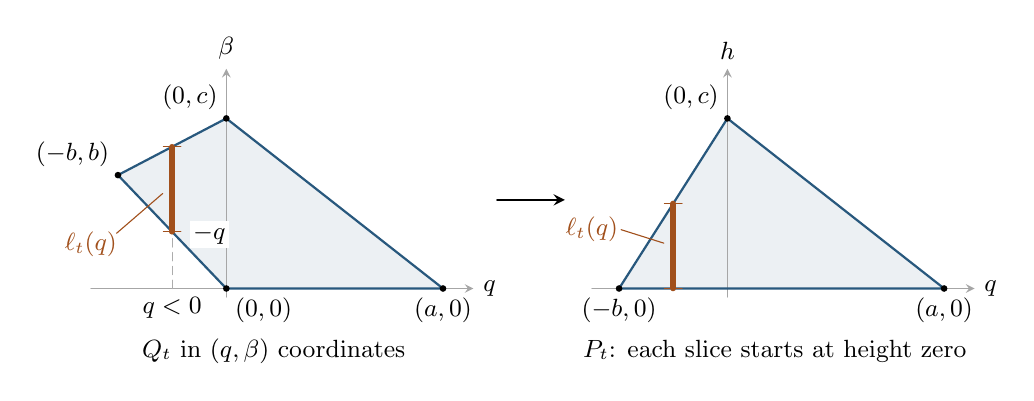
\begin{tikzpicture}[x=.86cm,y=.90cm,font=\small,
  line cap=round,line join=round,>=stealth]
  \definecolor{diagramblue}{RGB}{40,88,125}
  \definecolor{diagramorange}{RGB}{161,80,28}
  \begin{scope}
    \fill[diagramblue!9] (0,0)--(3.2,0)--(0,2.4)--(-1.6,1.6)--cycle;
    \draw[->,gray!70] (-2.0,0)--(3.65,0) node[right,text=black] {$q$};
    \draw[->,gray!70] (0,-.12)--(0,3.1) node[above,text=black] {$\beta$};
    \draw[diagramblue,thick] (0,0)--(3.2,0)--(0,2.4)--(-1.6,1.6)--cycle;
    \draw[densely dashed,gray!65] (-.8,0)--(-.8,.8);
    \draw[diagramorange,line width=2pt] (-.8,.8)--(-.8,2.0);
    \draw[diagramorange] (-.93,.8)--(-.67,.8) (-.93,2.0)--(-.67,2.0);
    \node[diagramorange] at (-2.0,.62) {$\ell_t(q)$};
    \draw[diagramorange,thin] (-1.62,.78)--(-.94,1.34);
    \node[anchor=west,fill=white,inner sep=1.3pt] at (-.55,.76) {$-q$};
    \fill (0,0) circle (1.2pt) (3.2,0) circle (1.2pt)
          (0,2.4) circle (1.2pt) (-1.6,1.6) circle (1.2pt);
    \node[below right,inner sep=3pt] at (0,0) {$(0,0)$};
    \node[below,inner sep=3pt] at (3.2,0) {$(a,0)$};
    \node[above left,inner sep=3pt] at (0,2.4) {$(0,c)$};
    \node[above left,inner sep=3pt] at (-1.6,1.6) {$(-b,b)$};
    \node[below,inner sep=3pt] at (-.8,0) {$q<0$};
    \node[align=center] at (.7,-.88) {$Q_t$ in $(q,\beta)$ coordinates};
  \end{scope}
  \draw[->,thick] (4.0,1.25)--(5.0,1.25);
  \begin{scope}[shift={(7.4,0)}]
    \fill[diagramblue!9] (-1.6,0)--(3.2,0)--(0,2.4)--cycle;
    \draw[->,gray!70] (-2.0,0)--(3.65,0) node[right,text=black] {$q$};
    \draw[->,gray!70] (0,-.12)--(0,3.1) node[above,text=black] {$h$};
    \draw[diagramblue,thick] (-1.6,0)--(3.2,0)--(0,2.4)--cycle;
    \draw[diagramorange,line width=2pt] (-.8,0)--(-.8,1.2);
    \draw[diagramorange] (-.93,0)--(-.67,0) (-.93,1.2)--(-.67,1.2);
    \node[diagramorange] at (-2.0,.83) {$\ell_t(q)$};
    \draw[diagramorange,thin] (-1.57,.83)--(-.94,.64);
    \fill (-1.6,0) circle (1.2pt) (3.2,0) circle (1.2pt)
          (0,2.4) circle (1.2pt);
    \node[below,inner sep=3pt] at (-1.6,0) {$(-b,0)$};
    \node[below,inner sep=3pt] at (3.2,0) {$(a,0)$};
    \node[above left,inner sep=3pt] at (0,2.4) {$(0,c)$};
    \node[align=center] at (.7,-.88) {$P_t$: each slice starts at height zero};
  \end{scope}
\end{tikzpicture}
\caption{Diagonal compression of exponent slices. For $c(a+b)>ab$, the
change $q=\alpha-\beta$ turns $Q_t$ into the quadrilateral on the left.
Moving each vertical slice down to height zero gives $P_t$, with the
same slice length $\ell_t(q)$. The highlighted slice has $q<0$ and lower
endpoint $-q$. This diagram describes the containing regions; the jet
transfer is proved by convergence of finite jet matrices.}
\label{fig:compression}
\end{figure}



\begin{proposition}[Diagonal compression]\label{prop:compression}
Let $k,m,r$ be positive integers.  If $\mathcal M(kP_t)$ has injective
order-$m$ jets at some $r$ distinct points of $\T$, then
$\mathcal M(kQ_t)$ has injective order-$m$ jets at some $r$ distinct
points of $\T$.
\end{proposition}

\begin{proof}
Use the torus coordinates
\[
 (x,z)=(u,v/u),\qquad (u,v)=(x,xz).
\]
A monomial $x^\alpha z^\beta$ becomes $u^qv^\beta$, where
$q=\alpha-\beta$.  For every nonempty integer slice $q$ of $kQ_t$, write
\[
 \beta_q^-=
 \min\{\beta\in\Z:(q+\beta,\beta)\in kQ_t\},
 \qquad
 \beta_q^+=
 \max\{\beta\in\Z:(q+\beta,\beta)\in kQ_t\}.
\]
Convexity of the slice implies that all integers between these endpoints
occur.  Hence the slice has the basis
\begin{equation}\label{eq:compression-row-basis}
 u^qv^{\beta_q^-}(v-1)^h,
 \qquad 0\le h\le\beta_q^+-\beta_q^-.
\end{equation}
Indeed, expanding $(v-1)^h$ gives a triangular change of basis from the
consecutive powers of $v$, with diagonal entries equal to one.  By Lemma~\ref{lem:slices},
\[
 h\le\beta_q^+-\beta_q^-
 \le k\ell_t(q/k).
\]
Consequently every pair $(q,h)$ in
\eqref{eq:compression-row-basis} belongs to $kP_t\cap\Z^2$.
These pairs are distinct, both within each slice and between different slices.

Let $(u_i,y_i)$, $1\le i\le r$, be distinct torus points giving an
injective jet test for $\mathcal M(kP_t)$, now written in the variables
$(u,y)$.  For a positive parameter $s$, substitute $v=1+sy$ into
\eqref{eq:compression-row-basis} and divide its member indexed by $h$
by $s^h$.  The resulting functions are
\begin{equation}\label{eq:compression-limit}
 u^q(1+sy)^{\beta_q^-}y^h
 \longrightarrow u^qy^h
 \qquad (s\longrightarrow0^+).
\end{equation}
The convergence is locally uniform, with every spatial derivative, on
fixed neighborhoods of the finitely many test points.  To see this,
choose bounded neighborhoods on which $u$ stays away from zero and
then take $s$ small enough that $|sy|<1/2$ there.  The factors
$(1+sy)^{\beta_q^-}$ are holomorphic and converge uniformly to one on
slightly larger neighborhoods, so the derivative assertion follows
from the Cauchy estimates.  The argument also applies to negative
Laurent powers, since $1+sy$ stays away from zero.

The distinct limiting monomials in \eqref{eq:compression-limit} span
a subspace of $\mathcal M(kP_t)$, so their jet matrix has full column
rank.  Lemma~\ref{lem:rank-persistence} gives the same conclusion for
the functions on the left for every sufficiently small positive $s$.
These functions form a rescaled pullback of a basis of
$\mathcal M(kQ_t)$.

For such an $s$, the corresponding points in the original torus are
\[
 \left(u_i,\frac{1+sy_i}{u_i}\right),\qquad 1\le i\le r.
\]
They lie in $\T$ because $u_i\ne0$ and $1+sy_i\ne0$.  They are distinct:
equality of two images forces equality first of their $u$ coordinates
and then of their $y$ coordinates.  The coordinate map
\[
 (u,y)\longmapsto\left(u,\frac{1+sy}{u}\right)
\]
has Jacobian determinant $s/u\ne0$, and therefore preserves orders of
vanishing at these points.  The full-column-rank conclusion is thus
exactly the required injectivity for $\mathcal M(kQ_t)$.
\end{proof}

The two transfers now give the test needed on the surface.

\begin{corollary}[From the triangle to the surface]
\label{cor:surface-transfer}
Let $k,m,r$ be positive integers.  If $\mathcal M(kP_t)$ has injective
order-$m$ jets at some $r$ distinct torus points, then $H^0(S,kL)$ has
injective order-$m$ jets at some $r$ distinct points of $S$.
\end{corollary}

\begin{proof}
If $H^0(S,kL)=0$, the conclusion is immediate.  Otherwise,
Proposition~\ref{prop:compression} gives such a jet test for
$\mathcal M(kQ_t)$.  Trivialize $L$ in the fixed coordinate chart at
the node and regard the sections of $kL$ as holomorphic germs there.
This identification is injective: a global section vanishing on a
nonempty open subset of the integral surface vanishes identically.
Proposition~\ref{prop:quadrilateral} gives a basis whose distinct
initial monomials lie in $kQ_t$.  Their span therefore has injective
jets at the torus tuple just constructed.  Applying
Proposition~\ref{prop:initial-transfer} gives injective jets for the
section germs at distinct points in the chart, and hence for
$H^0(S,kL)$ on $S$.
\end{proof}

\section{Finite subgroups as jet tests}\label{sec:lattice}

We now find an injective jet test for the triangle spaces
$\mathcal M(kP_t)$.  The test points will form a finite subgroup of the
complex torus.  Averaging over this group separates a Laurent polynomial
into components supported on cosets of a sublattice.  In the coordinates
of that sublattice, each component lies in a triangle for which a
one-point multiplicity estimate applies.

\subsection{A multiplicity estimate for triangles}

For a bounded subset of $\R^2$, its \emph{vertical range} is the length of
its projection onto the second coordinate axis.  The following estimate
allows arbitrary real vertices and translations.

\begin{lemma}\label{lem:triangle-multiplicity}
Let $\rho>0$, and let $\Delta\subset\R^2$ be a triangle of area
$\rho^2/2$ and vertical range $\rho$.  Every nonzero Laurent polynomial
$F\in\C[U^{\pm1},Z^{\pm1}]$ whose exponent support is contained in
$\Delta$ satisfies
\[
 \ord_{(1,1)}F\leq\rho.
\]
\end{lemma}

\begin{figure}[htbp]
\centering
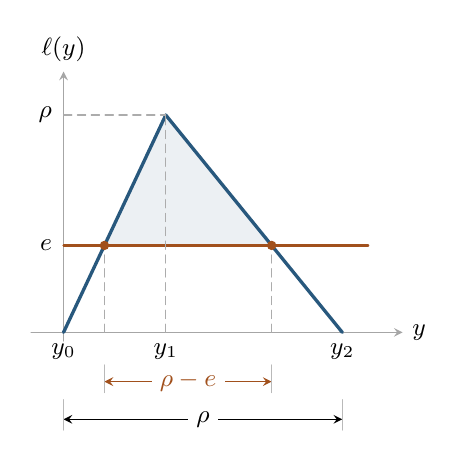
\begin{tikzpicture}[x=1.18cm,y=.92cm,font=\small,
  line cap=round,line join=round,>=stealth]
  \definecolor{sliceblue}{RGB}{40,88,125}
  \definecolor{sliceorange}{RGB}{161,80,28}
  \fill[sliceblue!9] (.44,1.2)--(1.1,3)--(2.24,1.2)--cycle;
  \draw[->,gray!70] (-.35,0)--(3.65,0) node[right,text=black] {$y$};
  \draw[->,gray!70] (0,-.12)--(0,3.6) node[above,text=black] {$\ell(y)$};
  \draw[sliceblue,very thick] (0,0)--(1.1,3)--(3,0);
  \draw[densely dashed,gray!65] (0,3)--(1.1,3);
  \draw[sliceorange,thick] (0,1.2)--(3.28,1.2);
  \draw[densely dashed,gray!65] (.44,0)--(.44,1.2)
    (2.24,0)--(2.24,1.2) (1.1,0)--(1.1,3);
  \fill[sliceorange] (.44,1.2) circle (1.7pt) (2.24,1.2) circle (1.7pt);
  \node[left,inner sep=4pt] at (0,3) {$\rho$};
  \node[left,inner sep=4pt] at (0,1.2) {$e$};
  \node[below,inner sep=4pt] at (0,0) {$y_0$};
  \node[below,inner sep=4pt] at (1.1,0) {$y_1$};
  \node[below,inner sep=4pt] at (3,0) {$y_2$};
  \draw[<->,sliceorange] (.44,-.68)--(2.24,-.68)
    node[midway,fill=white,inner sep=3pt] {$\rho-e$};
  \draw[gray!55] (.44,-.45)--(.44,-.83) (2.24,-.45)--(2.24,-.83);
  \draw[<->] (0,-1.20)--(3,-1.20)
    node[midway,fill=white,inner sep=3pt] {$\rho$};
  \draw[gray!55] (0,-.93)--(0,-1.35) (3,-.93)--(3,-1.35);
\end{tikzpicture}
\caption{Horizontal slice lengths of a triangle of area $\rho^2/2$
and vertical range $\rho$. The tent has height $\rho$. For
$0\le e\le\rho$, the heights in the vertical projection at which
$\ell(y)\ge e$ form an interval of length $\rho-e$.
The graph shows three distinct vertex heights; a horizontal side gives
the same conclusion with a one-sided tent.}
\label{fig:triangle-slices}
\end{figure}


\begin{proof}
For a height $y$ in the vertical projection of $\Delta$, let $\ell(y)$
be the horizontal length of the slice of $\Delta$ at that height.  Write
$y_0\leq y_1\leq y_2$ for the three vertex heights; thus
$y_2-y_0=\rho$.  If these heights are distinct, $\ell$ increases linearly
from zero at $y_0$ to its maximum at $y_1$, then decreases linearly to
zero at $y_2$.  If two vertex heights coincide, $\Delta$ has a horizontal
side and there is just one linear segment.  In either case, the area is
one half the vertical range times the maximum slice length.  The maximum
is therefore $\rho$.

More precisely, for $0\leq e\leq\rho$, the heights with
$\ell(y)\geq e$ form an interval of length $\rho-e$
(Figure~\ref{fig:triangle-slices}).  When the three
heights are distinct, its endpoints are
\[
 y_0+\frac e\rho(y_1-y_0),
 \qquad
 y_2-\frac e\rho(y_2-y_1).
\]
The same formulas apply when two adjacent heights coincide, including
the cases $e=0$ and $e=\rho$.

Write $F=\sum_q f_q(U)Z^q$, with each displayed row $f_q$ nonzero, and
let $e$ be the least order of these rows at $U=1$.  Dividing every row by
$(U-1)^e$ gives
\[
 F=(U-1)^eD,
 \qquad D=\sum_q d_q(U)Z^q,
 \qquad D(1,Z)\ne0.
\]
Indeed, at least one $d_q(1)$ is nonzero, and distinct powers of $Z$ are
linearly independent.  All $d_q$ remain Laurent polynomials, including
when some exponents are negative.

The horizontal exponent span of the row
$f_q=(U-1)^e d_q$ is exactly $e$ plus that of $d_q$: the extreme
coefficients of the product are nonzero.  Thus $\ell(q)\geq e$ for every
height occurring in $D$.  There is no cancellation between distinct
heights, since the multiplying factor depends only on $U$.  It follows
that $e\leq\rho$ and that the heights occurring in $D$ span an interval
of length at most $\rho-e$.

On setting $U=1$, some rows may disappear, but no new height appears.
The nonzero Laurent polynomial $D(1,Z)$ therefore has exponent span at
most $\rho-e$.  Multiplication by a power of $Z$, which is a unit at
$Z=1$, turns it into an ordinary polynomial of degree at most
$\rho-e$.  Consequently
\[
 \ord_{(1,1)}D
 \leq \ord_1 D(1,Z)
 \leq \rho-e.
\]
The first inequality holds because restriction cannot introduce a term
of smaller total degree into the local Taylor series.  Orders add under
products of nonzero holomorphic germs, so $\ord_{(1,1)}F\leq\rho$.
All exponent spans and orders used here are integers; no integrality of
$\rho$, the vertices, or the translating vector is required.
\end{proof}


\subsection{The subgroup test}

For integer vectors $u,\xi\in\Z^2$, write $\det(u,\xi)$ for their
oriented determinant, extending this notation linearly to real $\xi$.
A vector in $\Z^2$ is \emph{primitive} if its coordinates are coprime.

\begin{proposition}\label{prop:subgroup-test}
Let $H>0$, let $r$ be a positive integer, and let $P\subset\R^2$ be a
triangle of area $H/2$.  Suppose there is a primitive vector $u\in\Z^2$
such that
\[
 \max_{\xi\in P}\det(u,\xi)
 -\min_{\xi\in P}\det(u,\xi)=\sqrt{rH}.
\]
Then there is a subgroup $G\subset\T$ of exactly $r$ distinct points
such that, for all positive integers $k,m$ with
$m>k\sqrt{H/r}$, the order-$m$ jet test on $\mathcal M(kP)$ at $G$ is
injective.
\end{proposition}

\begin{proof}
Complete $u$ to an integer basis $(u,v_0)$ with $\det(u,v_0)=1$.
Put $v=rv_0$ and
\[
 M=\Z u+\Z v\subset\Z^2.
\]
This sublattice has index $r$.  For $\eta=(\eta_1,\eta_2)\in\Z^2$,
write $\chi_\eta(x,z)=x^{\eta_1}z^{\eta_2}$ for the corresponding
character on $\T$, and define
\[
 G=\{p\in\T:\chi_\eta(p)=1\text{ for every }\eta\in M\}.
\]
The characters $X=\chi_u$ and $Y=\chi_{v_0}$ are torus coordinates:
their exponent matrix is unimodular, so its inverse also has integer
entries.  In these coordinates,
\[
 G=\{(X,Y):X=1,\ Y^r=1\}.
\]
Over $\C$, this consists of exactly $r$ distinct points.

Suppose, toward a contradiction, that a nonzero
$f\in\mathcal M(kP)$ has order at least $m$ at every point of $G$.
For $g\in G$, let $(\tau_gf)(p)=f(gp)$.  Translation by $g$ permutes
$G$ and is locally invertible, so every $\tau_gf$ has the same prescribed
vanishing.  For a coset $\eta+M$, its character projection is
\[
 f_\eta=\frac1r\sum_{g\in G}\chi_\eta(g)^{-1}\tau_gf.
\]
This is exactly the sum of the monomials of $f$ with exponents in
$\eta+M$.  Indeed, if $\xi-\eta=n u+\ell v_0$, then
$\chi_{\xi-\eta}$ restricts to $\zeta^\ell$ on $G$.  The sum over the
$r$th roots of unity gives
\[
 \frac1r\sum_{g\in G}\chi_{\xi-\eta}(g)
 =\begin{cases}
 1,&\xi-\eta\in M,\\
 0,&\xi-\eta\notin M.
 \end{cases}
\]
Thus the displayed projection keeps precisely the required coset.
Each $f_\eta$ still has order at least $m$ at every point of $G$, and its
support remains inside $kP$.  Since the components sum to $f$, choose
one that is nonzero.

Multiplication by the Laurent monomial $\chi_{-\eta}$ preserves local
orders and shifts this component's support into $M$.  There is therefore
a nonzero Laurent polynomial $F$ such that
\[
 \chi_{-\eta}f_\eta=F(U,Z),
 \qquad U=\chi_u,
 \qquad Z=\chi_v=Y^r.
\]
The map $(x,z)\mapsto(U,Z)$ is locally invertible at the identity:
in coordinates $(X,Y)$ it is $(X,Y)\mapsto(X,Y^r)$, whose derivative at
$(1,1)$ is $\operatorname{diag}(1,r)$.  The complex inverse function theorem therefore makes it a biholomorphism
on sufficiently small analytic neighborhoods.  In particular,
\[
 \ord_{(1,1)}F
 =\ord_{(1,1)}(\chi_{-\eta}f_\eta)\geq m.
\]
Only local invertibility is used; the map need not be injective on the
whole torus.

Let $N$ be the matrix with columns $u,v$.  The exponent support of $F$
lies in the real triangle
\[
 \Delta=N^{-1}(kP-\eta).
\]
Since $\det N=r$, this triangle has area $k^2H/(2r)$.  The second
coordinate of $N^{-1}\xi$ is $\det(u,\xi)/r$, so its vertical range is
$k\sqrt{rH}/r=k\sqrt{H/r}$.  Translation by $\eta$ changes neither
calculation.  Lemma~\ref{lem:triangle-multiplicity}, with
$\rho=k\sqrt{H/r}$, now gives
$\ord_{(1,1)}F\leq k\sqrt{H/r}<m$, the required contradiction.
\end{proof}

\subsection{A direction for every sufficiently large integer}

We apply Proposition~\ref{prop:subgroup-test} to
\[
 P_t=\conv\{(-b,0),(a,0),(0,1/d)\},
 \qquad
 a=\frac{dHt}{1+t},\quad b=\frac{dH}{1+t},\quad t>T,
\]
with $d,H,T$ fixed in Section~\ref{sec:node}.  Every triangle in this
family has area $H/2$, since $a+b=dH$.  Varying $t$ continuously will
make its determinant projection have the exact length needed for each
large $r$.

\begin{lemma}\label{lem:direction}
Fix $d,H>0$ and $T>1$, and define $P_t$ as above for $t>T$.
For every sufficiently large integer $r$ there are $t>T$ and a primitive
vector $u\in\Z^2$ such that the range of $\det(u,\cdot)$ on $P_t$ has
length $\sqrt{rH}$.  The threshold depends only on $d,H,T$.
\end{lemma}

\begin{proof}
Put $W=dH$ and $a_0=WT/(1+T)$.  As $t$ ranges over $(T,\infty)$,
$a=Wt/(1+t)$ ranges continuously and bijectively over $(a_0,W)$.
For $R=\sqrt{rH}$ sufficiently large, choose $j$ to be the largest power
of two at most $R/(2W)$.  Then
\[
 \frac{R}{4W}<j\leq\frac{R}{2W},
 \qquad jW<R.
\]
The open interval
\[
 I_r=\bigl(d(R-jW),\ d(R-ja_0)\bigr)
\]
has length
\[
 dj(W-a_0)>\frac{dR}{4(1+T)},
\]
which exceeds $2$ for every sufficiently large $r$.  Hence $I_r$
contains an odd integer $i$.  Its lower endpoint is positive, so $i>0$;
as $j$ is a power of two, the vector $u=(i,j)$ is primitive.

The strict inequalities defining $I_r$ imply
\[
 a_*:=\frac{R-i/d}{j}\in(a_0,W).
\]
Choose the unique $t>T$ for which $a=a_*$.  Since $b=W-a$, we have
\[
 \frac{i}{d}+ja=R,
 \qquad
 \frac{i}{d}-jb=R-jW>0.
\]
The determinant functional has the three vertex values
\[
 \det\bigl(u,(-b,0)\bigr)=jb,
 \qquad
 \det\bigl(u,(a,0)\bigr)=-ja,
 \qquad
 \det\bigl(u,(0,1/d)\bigr)=\frac{i}{d}.
\]
Its minimum is therefore $-ja$ and its maximum is $i/d$, giving the
required range $R$ exactly.  All lower bounds on $r$ in this construction
depend only on the fixed data $d,H,T$.
\end{proof}

\begin{corollary}\label{cor:torus-test}
For the fixed parameters $d,H,T$ of Section~\ref{sec:node}, there is an
integer $r_0$ such that for every integer $r\geq r_0$ one can choose a
single $t>T$ and a subgroup $G\subset\T$ of $r$ distinct points for
which the following holds: for all positive integers $k,m$ satisfying
\[
 m>k\sqrt{H/r},
\]
the order-$m$ jet test on $\mathcal M(kP_t)$ at $G$ is injective.
\end{corollary}

\begin{proof}
First fix $r$ and choose $t$ and $u$ by Lemma~\ref{lem:direction}.
The area of $P_t$ is $H/2$, so Proposition~\ref{prop:subgroup-test}
produces $G$ with the stated property simultaneously for all $k,m$.
Thus $r_0$, and then $t,G$, are chosen before these two jet parameters.
\end{proof}

Corollary~\ref{cor:surface-transfer} now gives a surface configuration
with the same injective jet test for each pair $k,m$.  These configurations
may depend on the pair.  The next section passes to very general points
where all the tests hold at once, and uses them to prove nefness.

\section{From homogeneous jets to nefness}\label{sec:nef}

The preceding sections produce an injective jet test at some tuple for
each pair of integers $k,m$ above the critical slope. We first make all
these tests hold at one very general tuple. A separate surface argument
then converts them into inequalities for every curve, including curves
whose multiplicities at the points are unequal.

\begin{lemma}[The open locus of an injective jet test]\label{lem:jet-open}
Let $S$ be a smooth integral complex projective surface, let $L$ be a line
bundle, and let $r,k,m$ be positive integers. In the configuration space
\[
 U_r=\{(p_1,\ldots,p_r)\in S^r:p_i\ne p_j\text{ for }i\ne j\},
\]
the tuples at which the order-$m$ jet test on $H^0(S,L^{\otimes k})$
is injective form a Zariski-open subset. If each test in a countable
collection with fixed $S,L,r$ is injective at some tuple, then all those tests are
simultaneously injective at very general tuples. Their common locus is
nonempty.
\end{lemma}

\begin{proof}
Let $q_1,q_2:S\times S\to S$ be the projections and let
$\mathcal I_\Delta$ be the ideal of the diagonal. The bundle of jets
of orders less than $m$ is
\[
 \mathcal J_{k,m}
 =q_{1*}\!\left(q_2^*L^{\otimes k}\otimes
       \mathcal O_{S\times S}/\mathcal I_\Delta^m\right).
\]
This is the algebraic principal-parts construction
\cite[Tags 0G3P and 0638]{Stacks}; it is locally free of rank
$\binom{m+1}{2}$.
Indeed, the diagonal is a regular embedding with conormal bundle
$\Omega_S^1$; the successive quotients of the displayed sheaf, pushed
forward to $S$, are
$L^{\otimes k}\otimes\operatorname{Sym}^j\Omega_S^1$ for
$0\le j<m$. They are locally free of ranks $j+1$.
The thickened diagonal is finite over $S$, so these pushforwards are
exact and give the asserted filtration. The fiber at $p$ is
$(L^{\otimes k})_p/\mathfrak m_p^m(L^{\otimes k})_p$.

Writing $\operatorname{pr}_i:U_r\to S$ for the coordinate projections,
consider the algebraic bundle map
\[
 H^0(S,L^{\otimes k})\otimes\mathcal O_{U_r}
 \longrightarrow\bigoplus_{i=1}^r\operatorname{pr}_i^*\mathcal J_{k,m}.
\]
Its fiber kernel consists exactly of sections vanishing to order at
least $m$ at every point. If $n=h^0(S,L^{\otimes k})>0$, failure of
injectivity is cut out locally by the $n\times n$ minors. If $n=0$,
the map is injective everywhere. In either case the injective locus
is Zariski open, and a single injective tuple makes it nonempty.
The analytic and algebraic finite jets agree at complex points:
in local coordinates both are the same Taylor polynomial modulo terms
of total degree at least $m$. Thus a tuple obtained by the analytic
transfers of the preceding sections is a valid witness here.

The variety $U_r$ is smooth and irreducible. A proper algebraic closed
subset has empty interior in its complex manifold of points. For a
countable collection of nonempty injective loci, their complements are
therefore closed nowhere-dense subsets of $U_r(\C)$. This locally
compact Hausdorff space is a Baire space, so their common complement
is nonempty, indeed dense. By construction it is the complement of a
countable union of proper Zariski-closed subsets of $U_r$, as required
for very general tuples.
\end{proof}

We next record the precise Riemann--Roch argument that will turn a
negative curve into an effective divisor with equal prescribed
multiplicities. The divisor being made effective need not be nef.

\begin{lemma}[Effective multiples of a positive-square divisor]
\label{lem:positive-square}
Let $Y$ be a smooth integral complex projective surface, let $A$ be a
nef real divisor class, and let $D$ be a rational Cartier divisor.
If $D^2>0$ and $A\cdot D>0$, then
$H^0(Y,\mathcal O_Y(kD))\ne0$ for every sufficiently large positive
integer $k$ divisible by the denominators of $D$.
\end{lemma}

\begin{proof}
Choose a positive integer $q$ such that $qD$ is Cartier and let
$k$ run through positive multiples of $q$. By Serre duality \cite[Tag 0FVV, Lemma 48.27.1(6)--(7)]{Stacks},
\[
 h^2(Y,\mathcal O_Y(kD))
   =h^0(Y,\mathcal O_Y(K_Y-kD)).
\]
For sufficiently large $k$,
\[
 A\cdot(K_Y-kD)=A\cdot K_Y-kA\cdot D<0.
\]
A divisor with a nonzero section is linearly equivalent to an
effective divisor, which has nonnegative intersection with the nef
class $A$. Hence the displayed $h^2$ vanishes for all such $k$.
Surface Riemann--Roch \cite[Tag 02UO]{Stacks} now gives
\[
 \begin{split}
 h^0(Y,\mathcal O_Y(kD))
 &\ge \chi(Y,\mathcal O_Y(kD))\\
 &=\frac{k^2D^2-kD\cdot K_Y}{2}+\chi(Y,\mathcal O_Y)>0
 \end{split}
\]
for sufficiently large $k$, since $D^2>0$.
\end{proof}

\begin{proposition}[Homogeneous tests imply nefness]
\label{prop:homogeneous-nef}
Let $S$ be a smooth integral complex projective surface, let $L$ be
ample, and let $p_1,\ldots,p_r$ be distinct points. Put
$H=L^2$ and $w=\sqrt{H/r}$. Suppose that, for all positive integers
$k,m$ with $m>kw$, no nonzero section of $L^{\otimes k}$ vanishes to
order at least $m$ at every $p_i$. On the blow-up
$\pi:Y\to S$ of these points, with exceptional curves $E_i$, the real
divisor class
\[
 D_0=\pi^*L-w\sum_{i=1}^rE_i
\]
is nef.
\end{proposition}

\begin{proof}
Choose a Cartier divisor representing $L$ and retain the notation $L$
for it. Write $A=\pi^*L$ and $E=\sum_iE_i$. The class $A$ is nef and
\[
 A^2=H,\qquad A\cdot E_i=0,\qquad
 E_i\cdot E_j=-\delta_{ij},\qquad D_0^2=0.
\]
If $D_0$ were not nef, there would be an integral curve $C\subset Y$
with $D_0\cdot C<0$. Since $D_0\cdot E_i=w>0$, this curve is not
exceptional, and $A\cdot C=L\cdot\pi_*C>0$.
For sufficiently small positive rational $\delta$, both
\[
 (D_0-\delta C)^2=-2\delta D_0\cdot C+\delta^2C^2>0,
 \qquad
 A\cdot(D_0-\delta C)=H-\delta A\cdot C>0
\]
hold. Fix such a $\delta$. By continuity, there is a rational number
$s>w$, sufficiently close to $w$, such that
\[
 D=A-sE-\delta C
 \quad\text{satisfies}\quad D^2>0,\qquad A\cdot D>0.
\]
Here $A\cdot D=H-\delta A\cdot C$ is independent of $s$.

Choose a sufficiently large positive integer $k$ divisible by the
denominators of both $s$ and $\delta$.
Lemma~\ref{lem:positive-square} supplies an effective divisor
$F\sim kD$. Since $k\delta$ and $m=ks$ are positive integers,
\[
 F+k\delta C\sim kA-mE
\]
is effective. The blow-up identity \cite[Tag 0AGP, Lemma 54.3.4(4)]{Stacks}
\[
 \pi_*\mathcal O_Y(-mE)
   =\bigcap_{i=1}^r\mathcal I_{p_i}^{\,m}
\]
and the projection formula give a nonzero section of
$L^{\otimes k}$ vanishing to order at least $m$ at every $p_i$.
To recall the local content of this identity, sections of a pullback
line bundle descend across the missing points because $S$ is normal,
and the exceptional order of a local equation on the blow-up of a
smooth point is its ordinary multiplicity. Thus the condition at each
$E_i$ is precisely membership in $\mathcal I_{p_i}^{\,m}$.
But $m=ks>kw$, contradicting the hypothesis. Therefore $D_0$ is nef.
\end{proof}

For completeness, Riemann--Roch and a count of jet conditions also give
the universal upper bound for the Seshadri constant.

\begin{lemma}[The square upper bound]\label{lem:sesha-upper}
For every ample line bundle $L$ on a smooth integral complex projective
surface $S$ and every tuple of $r$ distinct points,
\[
 \varepsilon(S,L;p_1,\ldots,p_r)\le\sqrt{L^2/r}.
\]
\end{lemma}

\begin{proof}
Put $H=L^2$, let $\pi:Y\to S$ be the blow-up, and write
$A=\pi^*L$ and $E=\sum_iE_i$. Suppose $A-\lambda E$ is nef for
some $\lambda\ge0$. Fix $0<\alpha<\sqrt{H/r}$ and set
$m_k=\lceil k\alpha\rceil$. The proof of
Lemma~\ref{lem:positive-square}, applied on $S$ with $A=D=L$,
gives
\[
 h^0(S,L^{\otimes k})\ge \frac{H}{2}k^2+O(k).
\]
The dimension of the target of the order-$m_k$ jet evaluation at
the $r$ points is
\[
 r\binom{m_k+1}{2}=\frac{r\alpha^2}{2}k^2+O(k).
\]
Since $r\alpha^2<H$, evaluation has a nonzero kernel for all
sufficiently large $k$. A section in that kernel gives an effective
divisor $F_k\sim kA-m_kE$ on $Y$. Nefness implies
\[
 0\le(A-\lambda E)\cdot F_k=kH-\lambda r m_k.
\]
Letting $k\to\infty$ gives $\lambda\le H/(r\alpha)$, and then
letting $\alpha\uparrow\sqrt{H/r}$ gives
$\lambda\le\sqrt{H/r}$. Taking the supremum over the nef
coefficients $\lambda$ proves the claim.
\end{proof}

\begin{proof}[Proof of Theorem~\ref{thm:main}]
Choose the nodal divisor and parameters in
Section~\ref{sec:node}. Corollary~\ref{cor:torus-test} supplies an
integer $r_0$, depending only on these choices and hence on $(S,L)$,
with the following property. For every integer $r\ge r_0$, there is
a parameter $t>T$ and an $r$-point torus tuple such that the jet test
on $\mathcal M(kP_t)$ is injective for every pair of positive integers $k,m$
with $m>k\sqrt{H/r}$.

Fix any such integer $r$. For each of these pairs,
Corollary~\ref{cor:surface-transfer} gives an injective jet test on
$H^0(S,L^{\otimes k})$ at some tuple of $r$ distinct points of $S$.
The tuples may depend on $k,m$. Lemma~\ref{lem:jet-open} makes all
these countably many tests hold simultaneously at very general
tuples. Proposition~\ref{prop:homogeneous-nef} proves that the class
$\pi^*L-\sqrt{H/r}\sum_iE_i$ is nef at every such tuple.
Combining this lower bound for the Seshadri constant with
Lemma~\ref{lem:sesha-upper} proves the required equality.
The integer $r$ was arbitrary subject to $r\ge r_0$, and $r_0$
was fixed before $k,m$ were chosen. This proves the assertion for
every sufficiently large integer $r$.
\end{proof}

\subsection{Extension of the ground field}

\begin{corollary}\label{cor:fields}
Let $K$ be an uncountable algebraically closed field of characteristic
zero, let $S$ be a smooth integral projective surface over $K$, and let
$L$ be an ample line bundle on $S$. There is an integer $r_0=r_0(S,L)$
such that, for every $r\ge r_0$, outside a countable union of proper
Zariski-closed subsets of $U_r$, with nonempty complement, one has
\[
 \varepsilon(S,L;p_1,\ldots,p_r)=\sqrt{L^2/r}.
\]
\end{corollary}
\begin{proof}
Descend the projective equations and the finite gluing data for $L$ to
a subfield $F\subset K$ finitely generated over $\mathbb Q$. This gives
a smooth geometrically integral projective surface $S_0/F$ and an ample
line bundle $L_0$ whose base change is $(S,L)$; these properties descend
through field extension, and the finite-data descent and ampleness
criteria are recorded in \cite[Tags 01ZM and 0D3C]{Stacks}.
The field $F$ is countable and embeds into $\C$. Fix such an embedding
and choose $r_0$ from Theorem~\ref{thm:main} for $(S_{0,\C},L_{0,\C})$.
The intersection number $H=L_0^2=L^2$ is unchanged by field extension.

Fix $r\ge r_0$ and put $w=\sqrt{H/r}$. For every pair of positive
integers $a,m$ with $m>aw$, form on $U_{r,0}=U_r(S_0)$ the evaluation map
\[
 H^0(S_0,L_0^{\otimes a})\otimes\mathcal O_{U_{r,0}}
 \longrightarrow
 \bigoplus_{i=1}^r\operatorname{pr}_i^*\mathcal J_{a,m}
\]
using the principal-parts construction in the proof of
Lemma~\ref{lem:jet-open}. Its noninjectivity locus $B_{a,m}$ is closed,
cut out by maximal minors, and is empty if the source space is zero.
Principal parts and these minors commute with field extension, as does
$H^0$ by flat base change \cite[Tag 02KH]{Stacks}.
Each $B_{a,m}$ is proper over $\C$: at a tuple where
$A-wE$ is nef, with $A=\pi^*L_{0,\C}$ and $E=\sum_iE_i$, a section in
the evaluation kernel would give an effective divisor of class $aA-mE$,
whose intersection with $A-wE$ is $aH-rmw<0$.
Thus $B_{a,m}$ is proper over $F$ and remains proper over $K$.
The single threshold $r_0$ works for all these pairs.

Let $Z_r=\bigcup_{a,m:\,m>aw}B_{a,m,K}$. This is a countable union of
proper closed subsets. Its complement contains a $K$-point: the
function field $F(U_{r,0})$ has transcendence degree $2r$ over $F$ and
embeds over $F$ into $K$. Indeed, choose $2r$ algebraically independent
elements of $K$ over the countable field $F$ and extend the resulting
embedding of a rational function field across the finite algebraic
extension, using that $K$ is algebraically closed. The resulting
$K$-point maps to the generic point of $U_{r,0}$ and therefore avoids
all the $B_{a,m}$.

At every tuple outside $Z_r$, all the homogeneous jet tests are
injective. The proofs of Lemma~\ref{lem:positive-square},
Proposition~\ref{prop:homogeneous-nef}, and Lemma~\ref{lem:sesha-upper}
use only surface Riemann--Roch, Serre duality, and the blow-up ideal
identity, and are valid over $K$. They give nefness of
$\pi^*L-w\sum_iE_i$ and the matching upper bound, respectively.
\end{proof}

\bibliographystyle{alpha}
\begingroup
\small
\bibliography{references}
\endgroup
\end{document}
